\chapter{Miyazaki Hayao and Studio Ghibli: Spirits and the Environment}

\section{Studio Ghibli}

Studio Ghibli (\ja{スタジオジブリ}) was founded in 1985 by the directors
\textbf{Miyazaki Hayao} (\ja{宮崎駿}, b.\ 1941) and \textbf{Takahata Isao} (1935--2018)
with producer Suzuki Toshio, following the success of \emph{Nausicaä of the Valley of the
Wind} (1984). Its films are hand-drawn, carefully researched, and among the most
commercially successful films in Japanese history.

\begin{center}
\begin{tabular}{llp{7.5cm}}
\toprule
Film & Year & Supernatural elements \\
\midrule
\emph{Nausicaä} \ja{風の谷のナウシカ} & 1984 & giant insects (Ohmu) and a toxic forest that purifies a polluted earth \\
\emph{My Neighbor Totoro} \ja{となりのトトロ} & 1988 & forest spirit Totoro, Catbus, soot sprites \\
\emph{Pom Poko} \ja{平成狸合戦ぽんぽこ} & 1994 & shapeshifting tanuki vs.\ suburban development (Takahata) \\
\emph{Princess Mononoke} \ja{もののけ姫} & 1997 & animal gods, the Forest Spirit, kodama, curse-gods \\
\emph{Spirited Away} \ja{千と千尋の神隠し} & 2001 & bathhouse of the gods, No-Face, river spirit \\
\emph{Ponyo} \ja{崖の上のポニョ} & 2008 & fish-girl, sea goddess, tsunami \\
\bottomrule
\end{tabular}
\end{center}

\section{\emph{My Neighbor Totoro} (1988)}

\begin{itemize}
  \item Setting: rural Saitama (Tokorozawa) in the late 1950s. Two sisters, Satsuki and Mei,
        move to an old house with their father while their mother is in hospital
        (tuberculosis).
  \item The girls encounter \textbf{Totoro}, a huge furry forest spirit living in a giant
        camphor tree wrapped with a shimenawa rope (a sacred tree, Week 2), as well as
        \textbf{soot sprites} (\ja{まっくろくろすけ}, makkuro kurosuke) in the house and the
        \textbf{Catbus} (\ja{ネコバス}), a bakeneko reimagined as public transport.
  \item No one is evil. The spirits are protective and playful, and only children can see
        them.
\end{itemize}

\begin{important}[Totoro and nostalgia]
\begin{itemize}
  \item Totoro embodies \emph{satoyama} (\ja{里山}), the managed landscape of villages,
        rice paddies and woods, idealized as harmony between people and nature.
  \item The 1950s setting (just before high-speed growth) gives the film a nostalgic,
        \emph{furusato} quality, connecting to the yōkai boom of Week 8.
  \item Totoro is not a traditional yōkai but feels like one: Miyazaki invented a creature
        that ``could have been'' folklore. He became Ghibli's logo and a national icon;
        a Totoro forest trust preserves woodland near Tokorozawa.
\end{itemize}
\end{important}

\section{\emph{Princess Mononoke} (1997)}

\subsection{Setting and plot}

The film is set in the Muromachi period (14th--15th c.), but avoids samurai and court and
focuses on marginal people: the Emishi (an eastern people outside Yamato control), lepers,
ex-prostitutes working iron, and animal gods.

\begin{enumerate}
  \item \textbf{Ashitaka}, a young Emishi prince, kills a boar god transformed into a
        \emph{tatarigami} (curse-god) by an iron ball lodged in its body. The curse
        infects his arm.
  \item He travels west and finds \textbf{Irontown} (Tataraba), led by \textbf{Lady Eboshi},
        who employs outcasts, makes guns and clears the forest for iron sand.
  \item \textbf{San}, a human girl raised by the wolf god Moro, the ``mononoke
        princess'', fights Irontown to protect the forest.
  \item The \textbf{Forest Spirit} (Shishigami, \ja{シシ神}): by day a deer-like being with
        a human face that gives and takes life; by night the giant Night-Walker
        (Deidarabotchi).
  \item Eboshi shoots off the Forest Spirit's head for the emperor's agents; the headless
        spirit spreads death across the land until Ashitaka and San return the head. The
        forest regrows, but the old gods are gone.
\end{enumerate}

\begin{center}
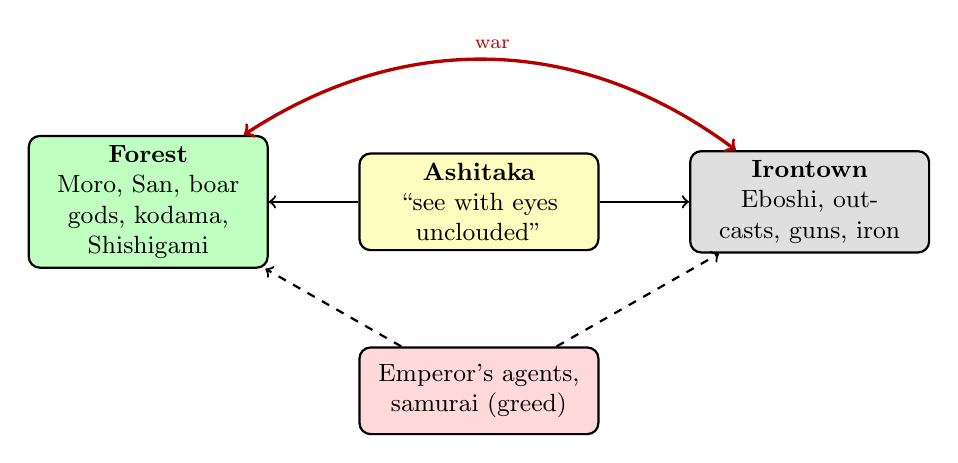
\begin{tikzpicture}[b/.style={draw, thick, rounded corners, align=center, font=\small, text width=2.8cm, minimum height=1.1cm}]
  \node[b, fill=green!25] (f) at (-4.2,0) {\textbf{Forest}\\Moro, San, boar gods, kodama, Shishigami};
  \node[b, fill=gray!25] (i) at (4.2,0) {\textbf{Irontown}\\Eboshi, outcasts, guns, iron};
  \node[b, fill=yellow!25] (a) at (0,0) {\textbf{Ashitaka}\\``see with eyes unclouded''};
  \node[b, fill=red!15] (e) at (0,-2.4) {Emperor's agents, samurai (greed)};
  \draw[<->, very thick, red!70!black] (f) to[bend left=35] node[above, font=\scriptsize] {war} (i);
  \draw[->, thick] (a) -- (f); \draw[->, thick] (a) -- (i);
  \draw[->, thick, dashed] (e) -- (i);
  \draw[->, thick, dashed] (e) -- (f);
\end{tikzpicture}
\end{center}

\begin{important}[Readings of \emph{Mononoke}]
\begin{itemize}
  \item \textbf{No simple villain}: Eboshi destroys the forest but liberates women and
        cares for lepers. Miyazaki refuses a nature-good / humans-bad binary.
  \item \textbf{Kami as dangerous}: the gods are not cute; they are huge, wild and
        vengeful, the ``rough spirit'' (aramitama) side of kami (Week 2).
  \item \textbf{Iron}: links to the Izumo iron culture of the Orochi myth (Week 3).
  \item \textbf{Mononoke}: the title uses the Heian word for possessing spirits (Week 4).
  \item \textbf{Revisionist history}: a Japan without the emperor at its centre, populated
        by Emishi and outcasts; influenced by historian Amino Yoshihiko.
\end{itemize}
\end{important}

\section{\emph{Spirited Away} (2001)}

\begin{center}
\begin{tabular}{ll}
\toprule
Japanese title & \ja{千と千尋の神隠し} (Sen to Chihiro no kamikakushi) \\
Literal meaning & ``The kamikakushi of Sen and Chihiro'' \\
Box office & highest-grossing film in Japan for nearly twenty years \\
Awards & Golden Bear (Berlin, 2002); Academy Award for Best Animated Feature (2003) \\
\bottomrule
\end{tabular}
\end{center}

\subsection{Plot}

Ten-year-old \textbf{Chihiro}, sulky about moving to a new town, wanders with her parents
through a tunnel into what looks like an abandoned theme park. Her parents eat food meant
for the gods and turn into pigs. Chihiro must work in a \textbf{bathhouse for the eight
million gods} run by the witch \textbf{Yubaba}, who takes her name and calls her
\textbf{Sen}. Helped by the boy \textbf{Haku}, she works, grows, helps a polluted river god
and the lonely spirit \textbf{No-Face} (\ja{カオナシ}, Kaonashi), remembers that Haku is the
spirit of a river (the Kohaku) that was filled in and built over, and rescues her parents.

\subsection{Folklore and themes}

\begin{itemize}
  \item \textbf{Kamikakushi} (\ja{神隠し}, ``hidden by the gods''): traditionally, children
        who disappeared were said to have been taken by kami or tengu (Week 6). Chihiro is
        literally spirited away.
  \item \textbf{Names}: losing your name means losing yourself; Yubaba controls workers by
        taking their names. This parallels the folk belief in the power of true names, and
        also modern labour (the bathhouse as a company).
  \item \textbf{Yomotsu-hegui}: eating food of the other world traps you there, as with
        Izanami in Yomi (Week 3). The parents' gluttony echoes the bubble era's
        consumerism.
  \item \textbf{Pollution and purification}: the ``stink spirit'' turns out to be a river god
        clogged with garbage (a bicycle, junk); when Chihiro pulls it out, he is purified.
        Purification (harae) is the central Shinto idea, applied to environmental pollution.
  \item \textbf{Bathhouse}: modelled on old public baths and the Dōgo Onsen; visiting
        gods come to rest as at a festival. The gods (a giant radish spirit, chick-like
        Otori-sama, kasuga masks) are drawn from folk religion and Miyazaki's imagination.
  \item \textbf{Coming of age}: Chihiro becomes capable and kind through work; Miyazaki said
        he made it for the ten-year-old daughters of his friends.
\end{itemize}

\begin{center}
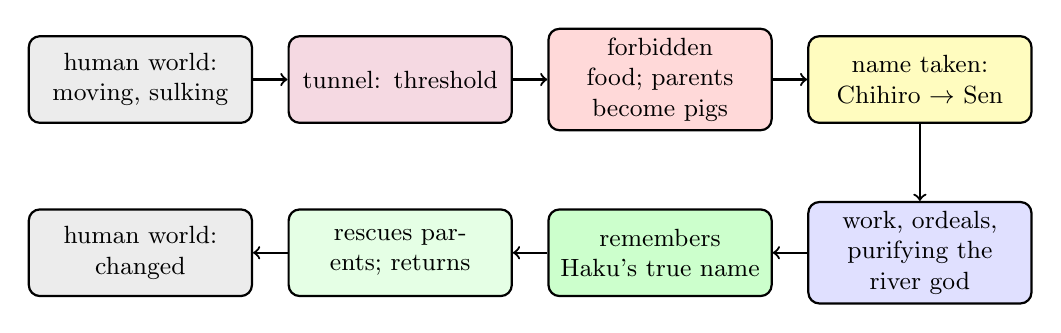
\begin{tikzpicture}[st/.style={draw, thick, rounded corners, align=center, font=\small, text width=2.6cm, minimum height=1.1cm}]
  \node[st, fill=gray!15] (1) at (0,0) {human world: moving, sulking};
  \node[st, fill=purple!15] (2) at (3.3,0) {tunnel: threshold};
  \node[st, fill=red!15] (3) at (6.6,0) {forbidden food; parents become pigs};
  \node[st, fill=yellow!25] (4) at (9.9,0) {name taken: Chihiro $\to$ Sen};
  \node[st, fill=blue!12] (5) at (9.9,-2.2) {work, ordeals, purifying the river god};
  \node[st, fill=green!20] (6) at (6.6,-2.2) {remembers Haku's true name};
  \node[st, fill=green!10] (7) at (3.3,-2.2) {rescues parents; returns};
  \node[st, fill=gray!15] (8) at (0,-2.2) {human world: changed};
  \draw[->, thick] (1) -- (2); \draw[->, thick] (2) -- (3); \draw[->, thick] (3) -- (4);
  \draw[->, thick] (4) -- (5); \draw[->, thick] (5) -- (6); \draw[->, thick] (6) -- (7);
  \draw[->, thick] (7) -- (8);
\end{tikzpicture}
\end{center}

\begin{remark}
The structure is a classic rite of passage (separation, liminal ordeal, reincorporation),
the same pattern as Izanagi's journey to Yomi or Urashima Tarō's visit to the Dragon
Palace. Unlike Izanagi, Chihiro obeys the final taboo: she does not look back as she
leaves the tunnel.
\end{remark}

\section{Miyazaki's spirit world: a synthesis}

\begin{center}
\begin{tabular}{p{3.5cm}p{9.5cm}}
\toprule
Traditional idea & Ghibli version \\
\midrule
kami in nature (animism) & Totoro in the camphor tree; kodama in the forest; Shishigami \\
rough/gentle aspects of kami & boar god as tatarigami; Forest Spirit gives and takes life \\
pollution and purification & stink spirit; the toxic jungle of \emph{Nausicaä} \\
kamikakushi & Chihiro's disappearance \\
bakeneko, tanuki & Catbus; \emph{Pom Poko} \\
fallen gods (Yanagita) & Haku, a river god who lost his river; the dying gods of \emph{Mononoke} \\
\bottomrule
\end{tabular}
\end{center}

\begin{aside}
Miyazaki has denied making ``Shinto films'', and calls himself more of an animist in a
loose sense. The professor's point: Ghibli does not illustrate a religion; it creates a
\emph{feeling} of a world full of spirits, which audiences then project back onto
``traditional Japan''. This is the same move Hearn and Yanagita made (Week 7).
\end{aside}

\section*{Summary}
\begin{itemize}
  \item Studio Ghibli (1985; Miyazaki, Takahata, Suzuki) made spirit-filled films that are
        central to how the world imagines Japanese religion and nature.
  \item \emph{Totoro}: benevolent forest spirit, satoyama nostalgia, the Catbus.
  \item \emph{Princess Mononoke}: Muromachi-era conflict between Irontown and dangerous
        animal gods; no simple villain.
  \item \emph{Spirited Away}: kamikakushi, names, forbidden food, pollution and
        purification, a rite of passage.
  \item Ghibli reworks folklore (kami, kamikakushi, fallen gods) into an
        environmentalist, humanist vision.
\end{itemize}
